\iffalse
\author{EE24BTECH11049}
\section{ee}
\chapter{2007}
\fi

%1st Question
    \item 
    The integral 
    \begin{align*}
        \frac{1}{2\pi} \int_0^{2\pi} \sin{\brak{t-\tau}}\cos{\tau}\, d\tau
    \end{align*}
    equals
    \hfill{\brak{\text{2007-EE}}}
    \begin{enumerate}
    \begin{multicols}{4}
        \item $\sin{t}\cos{t}$
        \item $0$
        \item $\frac{1}{2}\cos{t}$
        \item $\frac{1}{2}\sin{t}$
    \end{multicols}
    \end{enumerate}

    %2nd Question 
    \item 
    $X\brak{z} = 1 - 3z^{-1}$, $Y\brak{z} = 1 + 2z^{-2}$ are the Z-transforms of two signals $x\sbrak{n}$, $y\sbrak{n}$ respectively. A linear time invariant system has the impulse response $h\sbrak{n}$ defined by these two signals as 
    \begin{align*}
        h\sbrak{n} = x\sbrak{n-1} * y\sbrak{n}
    \end{align*}	
    where $*$ denotes discrete time convolution. Then the output of the system for the input $\delta\sbrak{n-1}$
    \hfill{\brak{\text{2007-EE}}}
    \begin{enumerate}
        \item has Z-transform $z^{-1}X\brak{z}y\brak{z}$
        \item equals $\delta\sbrak{n - 2} - 3\delta\sbrak{n - 3} + 2\delta\sbrak{n - 4} - 6\delta\sbrak{n - 5}$
        \item has Z-transform $1 - 3z^{-1} + 2z^{-2} - 6z^{-3} $ 
        \item does not satisfy any of the above three
    \end{enumerate}

    %3rd Question 
    \item 
    A loaded dice has the following probability distribution of occurrences

    \begin{table}[h!]    
      \centering
      \begin{tabular}{|c|c|c|c|c|c|c|}
        \hline
        \textbf{Dice Value} & 1 & 2 & 3 & 4 & 5 & 6 \\
        \hline
        \textbf{Probability} & $\frac{1}{4}$ & $\frac{1}{8}$ & $\frac{1}{8}$ & $\frac{1}{8}$ & $\frac{1}{8}$ & $\frac{1}{4}$ \\
        \hline
\end{tabular}
    \end{table}
    \hfill{\brak{\text{2007-EE}}}
    \begin{enumerate}
        \item same as the occurrence of 3, 4, 5
        \item same as the occurrence of 1, 2, 5
        \item $\frac{1}{128}$
        \item $\frac{5}{8}$
    \end{enumerate}

    %4th Question
    \item 
    let $x$ and $y$ be vectors in a three dimensional space and $\langle x,y\rangle$ denote their dot product. Then the determinant 
    \begin{align*}
        \text{det}\myvec{\langle x,x\rangle & \langle x,y\rangle \\ \langle y,x\rangle & \langle y,y\rangle} 
    \end{align*}
    \hfill{\brak{\text{2007-EE}}}
    \begin{enumerate}
        \item is zero when $x$ and $y$ are linearly independent
        \item is positive when $x$ and $y$ are linearly independent
        \item is non-zero for all  non-zero $x$ and $y$
        \item is zero when either of $x$ or $y$ is zero
    \end{enumerate}

    %5th Question 
    \item 
    The linear operater $L\brak{\vec{x}}$ is defined by the cross product $L\brak{\vec{x}} = \vec{b} \times \vec{x}$, where $\vec{b} = \myvec{0 & 1 & 0}^{T}$ and $\vec{x} = \myvec{x_1 & x_2 & x_3}^{T}$are three dimensional vectors. The $3 \times 3$ matrix $M$ of this operation satisfies 
    \begin{align*}
        L\brak{\vec{x}} = M\myvec{x_1 \\ x_2 \\ x_3}
    \end{align*}
    Then the eigenvalues of $M$ are
    \hfill{\brak{\text{2007-EE}}}
    \begin{enumerate}
    \begin{multicols}{4}
        \item $0, +1, -1$
        \item $1, -1, 1$
        \item $\iota, -\iota, 1$
        \item $\iota, -\iota, 0$
    \end{multicols}
    \end{enumerate}

    %6th Question
    \item 
    In the figure transformer $T_1$ has two secondaries, all three windings having same number turns and with polarities as indicated. One secondary is shorted by a $10\Omega$ resistor R, and the other by a $15 \mu F$ capacitor. The switch SW is opened $\brak{t = 0}$ when  the capacitor is charged to $5 V$ with the left plate as positive. At $t = 0+$ the voltage $V_P$ and the current $I_R$ are
    \begin{figure}[H]
        \centering
        \resizebox{0.5\textwidth}{!}{\begin{circuitikz}
	\tikzstyle{every node}=[font=\normalsize]
	\draw (2.75,9.75) to[battery1,l=$25V$] (2.75,6.75);
	\draw (2.75,9.75) to[opening switch,l={ \normalsize SW}] (4.25,9.75);
	\draw (4.25,9.75) to[R] (5.75,9.75);
	\draw (5.75,9.75) to[L ] (5.75,6.75);
	\draw (2.75,6.75) to[short] (5.75,6.75);
	\draw [->, >=Stealth] (5.5,7.5) -- (5.5,9)node[pos=0.5,left, fill=white]{$V_p$};
	\node at (5.5,9.25) [circ] {};
	\draw (7,9.75) to[L ] (7,8.5);
	\draw (7,8) to[L ] (7,6.75);
	\draw (8.75,8) to[C,l={ \normalsize $C$}] (7,8);
	\draw (7,8.5) to[short] (8.75,8.5);
	\draw (8.75,9.75) to[R,l={ \normalsize $R$}] (7,9.75);
	\draw (7,6.75) to[short] (8.75,6.75);
	\draw (8.75,9.75) to[short] (8.75,8.5);
	\draw (8.75,8) to[short] (8.75,6.75);
	\draw (6.25,9.75) to[short] (6.25,6.75);
	\node at (7.5,7) [circ] {};
	\draw (6.5,9.75) to[short] (6.5,6.75);
	\node [font=\normalsize] at (6.5,10) {$T_1$};
	\draw [->, >=Stealth] (7.25,10.25) -- (8.5,10.25)node[pos=0.5,above, fill=white]{$I_R$};
	\node at (7.5,9.25) [circ] {};
\end{circuitikz}
}
    \end{figure}
    \hfill{\brak{\text{2007-EE}}}
    \begin{enumerate}
        \item $-25V, 0.0A$
        \item very large voltage, very large current
        \item $5.0V, 0.5A$
        \item $-5.0V, -0.5A$
    \end{enumerate}

    %7th Question 
    \item 
    In the circuit of the adjacent figure the diode connects the ac source to a pure inductance L.
    The diode conducts for
    \begin{figure}[H]
    \centering
    \resizebox{0.3\textwidth}{!}{\begin{circuitikz}
	\tikzstyle{every node}=[font=\normalsize]
	\draw (2.75,6.5) to[sinusoidal voltage source, sources/symbol/rotate=auto,l={ \normalsize AC}] (2.75,8.75);
	\draw (2.75,8.75) to[D,l={ \normalsize D}] (5.25,8.75);
	\draw (5.25,6.5) to[L,l={ \normalsize Pure L} ] (5.25,8.75);
	\draw (2.75,6.5) to[short] (5.25,6.5);
\end{circuitikz}}
    \end{figure}
    \hfill{\brak{\text{2007-EE}}}
    \begin{enumerate}
    \begin{multicols}{4}
        \item $90^{\degree}$
        \item $180^{\degree}$
        \item $270^{\degree}$
        \item $360^{\degree}$
    \end{multicols}
    \end{enumerate}

    %8th Question
    \item 
    IC 555 in the adjacent figure is configured as an stable multivibrator. It is enabled to oscillate at $t = 0$ by applying a hight input to pin 4. The pin description is: 1 and 8-supply; 2-trigger; 4-reset; 6-threshold; 7-discharge. The waveform appearing across the capacitor starting from $t = 0$, as observed on storage CRO is
    \begin{figure}[H]
        \centering
        \resizebox{0.3\textwidth}{!}{\begin{circuitikz}
	\tikzstyle{every node}=[font=\large]
	\draw  (4.75,9.5) rectangle (8.25,4.75);
	\draw  (5.25,7.75) rectangle  node {\large IC 555} (7.75,6.75);
	\node at (6.5,4.75) [circ] {};
	\node at (5.75,4.75) [circ] {};
	\node at (6.5,9.5) [circ] {};
	\node at (4.75,5.5) [circ] {};
	\node at (4.75,8.5) [circ] {};
	\node [font=\large] at (8.5,7) {3};
	\node at (8.25,7) [circ] {};
	\node [font=\large] at (6.5,9) {8};
	\node [font=\large] at (6.5,5) {1};
	\node [font=\large] at (5.75,5) {4};
	\node [font=\large] at (5.1,5.5) {     2,6};
	\node [font=\large] at (5,8.5) {7};
	\draw (6.5,4.75) to (6.5,4.25) node[ground]{};
	\draw (3.75,8.25) to[european resistor,l={ \large 10K}] (3.75,10.25);
	\draw (3.75,6) to[european resistor,l={ \large 10K}] (3.75,8.25);
	\draw (3.75,4.25) to[C,l={ \large C}] (3.75,6);
	\draw [->, >=Stealth] (3.75,10.25) -- (3.75,11);
	\node [font=\large] at (4,11) {$+$};
	\draw (2.25,8.5) to[D] (2.25,5.5);
	\draw (2.25,8.5) to[short] (4.75,8.5);
	\draw (2.25,5.5) to[short] (4.75,5.5);
	\draw (3.75,10.5) to[short] (6.5,10.5);
	\draw (6.5,10.5) to[short] (6.5,9.5);
	\draw (3.75,4.25) to (3.75,4) node[ground]{};
	\draw (2.25,3) to[short] (5.75,3);
	\draw (5.75,4.75) to[short] (5.75,3);
	\draw (2.25,3.25) to[short] (2.75,3.25);
	\draw (2.75,3.25) to[short] (2.75,3.75);
	\draw (2.75,3.75) to[short] (3.25,3.75);
\end{circuitikz}
}
    \end{figure}
    \hfill{\brak{\text{2007-EE}}}
    \begin{multicols}{2}
    \begin{enumerate}
        \item 
        \begin{figure}[H]
        \centering
        \resizebox{0.25\textwidth}{!}{\begin{circuitikz}
\tikzstyle{every node}=[font=\large]
\draw (1.75,5) to[short] (6.75,5);
\draw (6.75,9) to[short] (6.75,5);
\draw (1.75,9) to[short] (6.75,9);
\draw (1.75,9) to[short] (1.75,5);
\draw (1.75,5.5) to[short] (6.75,5.5);
\draw (1.75,6) to[short] (6.75,6);
\draw (1.75,6.5) to[short] (6.75,6.5);
\draw (1.75,7) to[short] (6.75,7);
\draw (1.75,7.5) to[short] (6.75,7.5);
\draw (1.75,8) to[short] (6.75,8);
\draw (1.75,8.5) to[short] (6.75,8.5);
\draw (6.25,9) to[short] (6.25,5);
\draw (5.75,9) to[short] (5.75,5);
\draw (5.25,9) to[short] (5.25,5);
\draw (4.75,9) to[short] (4.75,5);
\draw (4.25,9) to[short] (4.25,5);
\draw (3.75,9) to[short] (3.75,5);
\draw (3.25,9) to[short] (3.25,5);
\draw (2.75,9) to[short] (2.75,5);
\draw (2.25,9) to[short] (2.25,5);
\draw [short] (1.75,5) -- (2.25,6);
\draw [short] (2.25,6) .. controls (2.75,7) and (2.75,7) .. (3.25,7);
\draw [short] (3.25,7) .. controls (3.5,6.5) and (3.5,6.25) .. (4.25,6);
\draw [short] (4.25,6) .. controls (4.5,6.75) and (4.5,7) .. (5.25,7);
\draw [short] (5.25,7) .. controls (5.5,6.5) and (5.5,6.25) .. (6.25,6);
\draw [short] (6.25,6) .. controls (6.25,6.5) and (6.5,6.75) .. (6.75,6.75);
\draw [ line width=1.6pt ] (1.75,9) rectangle (6.75,5);
\end{circuitikz}}
        \end{figure}

        \item 
        \begin{figure}[H]
        \centering
        \resizebox{0.25\textwidth}{!}{\begin{circuitikz}
    \tikzstyle{every node}=[font=\LARGE]
    \draw (3.5,9.5) to[short] (8.5,9.5);
    \draw (3.5,9) to[short] (8.5,9);
    \draw (3.5,8.5) to[short] (8.5,8.5);
    \draw (3.5,8) to[short] (8.5,8);
    \draw (3.5,7.5) to[short] (8.5,7.5);
    \draw (3.5,7) to[short] (8.5,7);
    \draw (3.5,6.5) to[short] (8.5,6.5);
    \draw (3.5,6) to[short] (8.5,6);
    \draw (3.5,5.5) to[short] (8.5,5.5);
    \draw (3.5,9.5) to[short] (3.5,5.5);
    \draw (8.5,9.5) to[short] (8.5,5.5);
    \draw (4,9.5) to[short] (4,5.5);
    \draw (4.5,9.5) to[short] (4.5,5.5);
    \draw (5,9.5) to[short] (5,5.5);
    \draw (5.5,9.5) to[short] (5.5,5.5);
    \draw (6,9.5) to[short] (6,5.5);
    \draw (6.5,9.5) to[short] (6.5,5.5);
    \draw (7,9.5) to[short] (7,5.5);
    \draw (7.5,9.5) to[short] (7.5,5.5);
    \draw (8,9.5) to[short] (8,5.5);
    \draw [line width=0.5pt, short] (3.5,6.5) .. controls (4,7.25) and (3.75,7.5) .. (4.5,7.5);
    \draw [line width=0.5pt, short] (4.5,7.5) .. controls (4.75,7) and (4.75,6.75) .. (5.5,6.5);
    \draw [line width=0.5pt, short] (5.5,6.5) .. controls (6,7.25) and (5.75,7.5) .. (6.5,7.5);
    \draw [line width=0.5pt, short] (6.5,7.5) .. controls (6.75,7) and (6.75,6.75) .. (7.5,6.5);
    \draw [line width=0.5pt, short] (7.5,6.5) .. controls (8,7.5) and (7.75,7.25) .. (8.5,7.5);
    \draw [ line width=1.6pt ] (3.5,9.5) rectangle (8.5,5.5);
\end{circuitikz}}
        \end{figure}

        \item 
        \begin{figure}[H]
        \centering
        \resizebox{0.25\textwidth}{!}{\begin{circuitikz}
\tikzstyle{every node}=[font=\large]
\draw (1.75,5) to[short] (6.75,5);
\draw (6.75,9) to[short] (6.75,5);
\draw (1.75,9) to[short] (6.75,9);
\draw (1.75,9) to[short] (1.75,5);
\draw (1.75,5.5) to[short] (6.75,5.5);
\draw (1.75,6) to[short] (6.75,6);
\draw (1.75,6.5) to[short] (6.75,6.5);
\draw (1.75,7) to[short] (6.75,7);
\draw (1.75,7.5) to[short] (6.75,7.5);
\draw (1.75,8) to[short] (6.75,8);
\draw (1.75,8.5) to[short] (6.75,8.5);
\draw (6.25,9) to[short] (6.25,5);
\draw (5.75,9) to[short] (5.75,5);
\draw (5.25,9) to[short] (5.25,5);
\draw (4.75,9) to[short] (4.75,5);
\draw (4.25,9) to[short] (4.25,5);
\draw (3.75,9) to[short] (3.75,5);
\draw (3.25,9) to[short] (3.25,5);
\draw (2.75,9) to[short] (2.75,5);
\draw (2.25,9) to[short] (2.25,5);
\draw [short] (1.75,5) .. controls (2,6.25) and (1.75,6.75) .. (2.75,7);
\draw [short] (2.75,7) .. controls (3.25,6.5) and (3.25,6.25) .. (4.25,6);
\draw [short] (4.25,6) .. controls (4.5,6.75) and (4.5,7) .. (5.25,7);
\draw [short] (5.25,7) .. controls (5.5,6.5) and (5.75,6.25) .. (6.75,6);
\draw [ line width=1.6pt ] (1.75,9) rectangle (6.75,5);
\end{circuitikz}}
        \end{figure}

        \item 
        \begin{figure}[H]
        \centering
        \resizebox{0.25\textwidth}{!}{\begin{circuitikz}
    \tikzstyle{every node}=[font=\LARGE]
    \draw (3.5,9.5) to[short] (8.5,9.5);
    \draw (3.5,9) to[short] (8.5,9);
    \draw (3.5,8.5) to[short] (8.5,8.5);
    \draw (3.5,8) to[short] (8.5,8);
    \draw (3.5,7.5) to[short] (8.5,7.5);
    \draw (3.5,7) to[short] (8.5,7);
    \draw (3.5,6.5) to[short] (8.5,6.5);
    \draw (3.5,6) to[short] (8.5,6);
    \draw (3.5,5.5) to[short] (8.5,5.5);
    \draw (3.5,9.5) to[short] (3.5,5.5);
    \draw (8.5,9.5) to[short] (8.5,5.5);
    \draw (4,9.5) to[short] (4,5.5);
    \draw (4.5,9.5) to[short] (4.5,5.5);
    \draw (5,9.5) to[short] (5,5.5);
    \draw (5.5,9.5) to[short] (5.5,5.5);
    \draw (6,9.5) to[short] (6,5.5);
    \draw (6.5,9.5) to[short] (6.5,5.5);
    \draw (7,9.5) to[short] (7,5.5);
    \draw (7.5,9.5) to[short] (7.5,5.5);
    \draw (8,9.5) to[short] (8,5.5);
    \draw [short] (3.5,6.5) .. controls (4,7.25) and (4,7.5) .. (5,7.5);
    \draw [short] (5,7.5) .. controls (5.25,6.75) and (5.25,6.75) .. (6,6.5);
    \draw [short] (6,6.5) .. controls (6.5,7.25) and (6.5,7.5) .. (7.5,7.5);
    \draw [short] (7.5,7.5) .. controls (7.75,6.75) and (7.75,6.75) .. (8.5,6.5);
    \draw  (3.5,9.5) rectangle (5.5,9.5);
    \draw [ line width=1.6pt ] (3.5,9.5) rectangle (8.5,5.5);
\end{circuitikz}}
        \end{figure}
    \end{enumerate}
\end{multicols}

    %9th Question 
    \item 
    The circuit in the figure is a current commutated dc - dc chopper where, $Th_M$ is the main SCR and $Th_{AUX}$ is the auxiliary SCR. The load current is constant at $t = 0$. $Th_M$ si turned OFF between 
    \begin{figure}[H]
    \centering
    \resizebox{0.45\textwidth}{!}{\begin{circuitikz}
	\tikzstyle{every node}=[font=\normalsize]
	\draw (2.25,8.25) to[battery2,l=$230V$] (2.25,4);
	\draw (2.25,8.25) to[short] (4.25,8.25);
	\draw (4.25,8.25) to[D,l={ \large $Th_{M}$}] (6.5,8.25);
	\draw (4.25,8.25) to[D] (4.25,7);
	\draw (4.25,7) to[D,l={ \large $Th_{AUX}$}] (6.5,7);
	\draw (5,6.25) to[C,l={ \normalsize $10\mu F$}] (4.25,6.25);
	\draw (6.5,6.25) to[L,l={ \normalsize $25.28\mu H$} ] (5,6.25);
	\draw (4.25,7) to[short] (4.25,6.25);
	\draw (6.5,8.25) to[short] (6.5,6.25);
	\draw (6.5,8.25) to[short] (8.5,8.25);
	\draw (2.25,4) to[short] (8.5,4);
	\draw (8.5,8.25) to[european resistor,l={ \normalsize LOAD}] (8.5,4);
	\draw (7.5,4) to[D] (7.5,8.25);
\end{circuitikz}
}
    \end{figure}
    \hfill{\brak{\text{2007-EE}}}
    \begin{enumerate}
        \item $0\mu s < t \leq 25\mu s$
        \item $25\mu s < t \leq 50\mu s$
        \item $50\mu s < t \leq 75\mu s$
        \item $75\mu s < t \leq 100\mu s$
    \end{enumerate}

    %10th question 
    \item 
    In the circuit shown in figure switch $SW_1$ is initially CLOSED and $SW_2$ is OPEN. The inductor L carries a current of $10 A$ and the capacitor is charged to $10V$ with polarities as indicated. $SW_2$ is initially CLOSED at $t = 0-$ and $SW_1$ is OPENED at $t = 0$. The current through C and the voltage across L at $t = 0+$ is

    \begin{figure}[H]
    \centering
    \resizebox{0.5\textwidth}{!}{\begin{circuitikz}
	\tikzstyle{every node}=[font=\normalsize]
	\draw (1.75,4.5) to[R,l={ \Large $R_1 = 10\Omega$}] (1.75,8.75);
	\draw (3.25,4.5) to[normal open switch,l={ \Large $SW_1$}] (3.25,8.75);
	\draw (4.75,4.5) to[L,l={ \Large L} ] (4.75,8.75);
	\draw (1.75,8.75) to[short] (4.75,8.75);
	\draw (4.75,8.75) to[normal open switch,l={ \Large $SW_2$}] (6.5,8.75);
	\draw (6.5,8.75) to[R,l={ \Large $R_2 = 10\Omega$}] (9.25,8.75);
	\draw (9.25,8.75) to[C,l={ \Large C }] (9.25,4.5);
	\draw (1.75,4.5) to[short] (9.25,4.5);
	\draw [->, >=Stealth] (5.5,6) -- (5.5,7.5)node[pos=0.5,right, fill=white]{$10A$};
	\node [font=\Large] at (9.75,6.25) {10V   };
\end{circuitikz}}
    \end{figure}
    \hfill{\brak{\text{2007-EE}}}
    \begin{enumerate}
    \begin{multicols}{4}
        \item $55A$, $4.5V$
        \item $5.5A$, $45V$
        \item $45A$, $5.5V$
        \item $4.5A$, $55V$
    \end{multicols}
    \end{enumerate}

    %11th Question 
    \item 
    The R-L-C series circuit shown is supplied from a variable frequency voltage source. The admittance-locus of the R-L-C network at terminals AB for increasing frequency $\omega$ is

    \begin{figure}[H]
        \centering
        \resizebox{0.3\textwidth}{!}{\begin{circuitikz}
	\tikzstyle{every node}=[font=\large]
	\draw (2,6) to[sinusoidal voltage source, sources/symbol/rotate=auto,l={ \large $\omega$}] (2,9);
	\draw (2,9) to[short] (3,9);
	\draw (2,6) to[short] (3,6);
	\draw (3,9) to[R,l={ \large R}] (5,9);
	\draw (3,6) to[C,l={ \large C}] (5,6);
	\draw (5,9) to[L,l={ \large L} ] (5,6);
	\node at (2.75,9) [circ] {};
	\node at (2.75,6) [circ] {};
	\node [font=\large] at (2.75,6.5) {B};
	\node [font=\large] at (2.75,8.5) {A};
\end{circuitikz}}
    \end{figure}
    \hfill{\brak{\text{2007-EE}}}
        \begin{multicols}{2}
        \begin{enumerate}  
        
        \item 
        \begin{figure}[H]
        \centering
        \resizebox{0.3\textwidth}{!}{\begin{circuitikz}
    \tikzstyle{every node}=[font=\normalsize]
    \draw (3.5,11.25) to[short] (3.5,7.5);
    \draw (3,9.5) to[short] (7.5,9.5);
    \draw  (4.5,9.5) circle (1cm);
    \draw [->, >=Stealth] (6.25,9.25) -- (7.5,9.25)node[pos=0.5,below, fill=white]{Re};
    \draw [->, >=Stealth] (3.25,10.5) -- (3.25,11.25)node[pos=0.5,left, fill=white]{Im};
    \draw [line width=2pt,->, >=Stealth] (4.5,8.5) -- (4.75,8.5);
    \node at (4.5,8.2) {$\omega$};
\end{circuitikz}}
        \end{figure}
        \item 
        \begin{figure}[H]
        \centering
        \resizebox{0.3\textwidth}{!}{\begin{circuitikz}
    \tikzstyle{every node}=[font=\normalsize]
    \draw (3.5,11.25) to[short] (3.5,7.5);
    \draw (3,9.5) to[short] (7.5,9.5);
    \draw  (4.5,9.5) circle (1cm);
    \draw [->, >=Stealth] (6.25,9.25) -- (7.5,9.25)node[pos=0.5,below, fill=white]{Re};
    \draw [->, >=Stealth] (3.25,10.25) -- (3.25,11.25)node[pos=0.5,left, fill=white]{Im};
    \draw [line width=2pt,->, >=Stealth] (4.5,8.5) -- (4.25,8.5);
    \node at (4.5,8.2) {$\omega$};
\end{circuitikz}}
        \end{figure}
        
        \item 
        \begin{figure}[H]
        \centering
        \resizebox{0.25\textwidth}{!}{\begin{circuitikz}
    \tikzstyle{every node}=[font=\normalsize]
    \draw (3.5,11.25) to[short] (3.5,7.5);
    \draw (1.5,8) to[short] (6,8);
    \draw [->, >=Stealth] (4.75,7.75) -- (6,7.75)node[pos=0.5,below, fill=white]{Re};
    \draw [->, >=Stealth] (3.25,10.25) -- (3.25,11.25)node[pos=0.5,left, fill=white]{Im};
    \draw  (3.5,9) circle (1cm);
    \draw [line width=2pt,->, >=Stealth] (4.5,9) --(4.5,9.25);
    \node at (4.7,9.25) {$\omega$};
\end{circuitikz}}
        \end{figure}
        

        \item 
        \begin{figure}[H]
        \centering
        \resizebox{0.25\textwidth}{!}{\begin{circuitikz}
    \tikzstyle{every node}=[font=\normalsize]
    \draw (3.5,11.25) to[short] (3.5,7.5);
    \draw (1.5,8) to[short] (6,8);
    \draw [->, >=Stealth] (4.75,7.75) -- (6,7.75)node[pos=0.5,below, fill=white]{Re};
    \draw [->, >=Stealth] (3.25,10.25) -- (3.25,11.25)node[pos=0.5,left, fill=white]{Im};
    \draw  (3.5,9) circle (1cm);
    \draw [line width=2pt, ->, >=Stealth] (2.5,9) -- (2.5,9.25);
    \node at (2.3,9.25) {$\omega$};
\end{circuitikz}}
        \end{figure}
        
        \end{enumerate}
        \end{multicols}

    %12th Question 
    \item 
    In the figure given below all phasors are with reference to the potential at point "O". The locus of voltage phasor $\vec{v_{XY}}$ as R is varied from zero to infinity is shown by 

    \begin{figure}[H]
    \centering
    \resizebox{0.35\textwidth}{!}{\begin{circuitikz}
\tikzstyle{every node}=[font=\normalsize]
\draw (2.5,9.75) to[sinusoidal voltage source, sources/symbol/rotate=auto] (2.5,8.25);
\draw (2.5,8.25) to[sinusoidal voltage source, sources/symbol/rotate=auto] (2.5,6.75);
\draw (2.5,8.25) to[short] (3,8.25);
\draw (3.75,8.25) to[short] (4.25,8.25);
\draw (4.25,9.75) to[european resistor,l={ \large R}] (4.25,8.25);
\draw (4.25,8.25) to[C,l={ \large C}] (4.25,6.75);
\draw (2.5,6.75) to[short] (4.25,6.75);
\draw (2.5,9.75) to[short] (4.25,9.75);
\node at (3,8.25) [squarepole] {};
\node at (3.75,8.25) [squarepole] {};
\draw [->, >=Stealth] (3.75,8.75) -- (4.75,9.5);
\draw [->, >=Stealth] (2,7.25) -- (2,8)node[pos=0.5,left, fill=white]{$V\angle 0^{\degree}$};
\draw [->, >=Stealth] (2,8.75) -- (2,9.5)node[pos=0.5,left, fill=white]{$V\angle 0^{\degree}$};
\draw [->, >=Stealth] (3,8.5) -- (3.75,8.5);
\node [font=\normalsize] at (3.4,8.8) {$V_{XY}$};
\node [font=\normalsize] at (3,8) {X};
\node [font=\normalsize] at (3.75,8) {Y};
\end{circuitikz}}
    \end{figure}
    \hfill{\brak{\text{2007-EE}}}
    \begin{multicols}{2}
    \begin{enumerate}
        \item  
        \begin{figure}[H]
        \centering
        \resizebox{0.4\textwidth}{!}{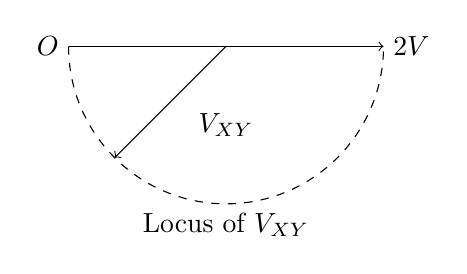
\begin{tikzpicture}
    \draw[dashed] (-2,0) arc[start angle=180, end angle=360, radius=2cm];
    \draw[->] (0,0) -- (-1.414, -1.414);
    \draw[->] (-2,0) -- (2,0);
    \node at (0,-1) {$V_{XY}$};
    \node at (-2,0) [left] {$O$};
    \node at (2,0) [right] {$2V$};
    \node at (0,-2) [below] {Locus of $V_{XY}$};
\end{tikzpicture}}
        \end{figure}

        \item  
        \begin{figure}[H]
        \centering
        \resizebox{0.4\textwidth}{!}{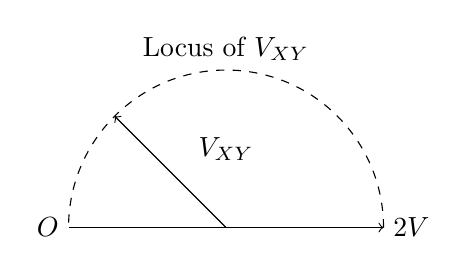
\begin{tikzpicture}
    \draw[dashed] (2,0) arc[start angle=0, end angle=180, radius=2cm];
    \draw[->] (0,0) -- (-1.414, 1.414);
    \draw[->] (-2,0) -- (2,0);
    \node at (0,1) {$V_{XY}$};
    \node at (-2,0) [left] {$O$};
    \node at (2,0) [right] {$2V$};
    \node at (0,2) [above] {Locus of $V_{XY}$};
\end{tikzpicture}}
        \end{figure}

        \item  
        \begin{figure}[H]
        \centering
        \resizebox{0.4\textwidth}{!}{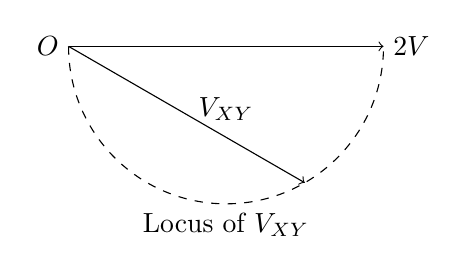
\begin{tikzpicture}
    \draw[dashed] (-2,0) arc[start angle=180, end angle=360, radius=2cm];
    \draw[->] (-2,0) -- (1, -1.732);
    \draw[->] (-2,0) -- (2,0);
    \node at (0,-0.8) {$V_{XY}$};
    \node at (-2,0) [left] {$O$};
    \node at (2,0) [right] {$2V$};
    \node at (0,-2) [below] {Locus of $V_{XY}$};
\end{tikzpicture}}
        \end{figure}

        \item  
        \begin{figure}[H]
        \centering
        \resizebox{0.4\textwidth}{!}{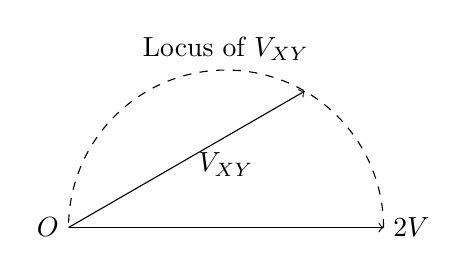
\begin{tikzpicture}
    \draw[dashed] (2,0) arc[start angle=0, end angle=180, radius=2cm];
    \draw[->] (-2,0) -- (1, 1.732);
    \draw[->] (-2,0) -- (2,0);
    \node at (0,0.8) {$V_{XY}$};
    \node at (-2,0) [left] {$O$};
    \node at (2,0) [right] {$2V$};
    \node at (0,2) [above] {Locus of $V_{XY}$};
\end{tikzpicture}}
        \end{figure}
    \end{enumerate}
    \end{multicols}

    %13th Question
    \item 
    A $3V$ dc supply with an internal resistance of $2\Omega$ supplies a passive non-linear resistance characterized by the relation $V_{NL} = I_{NL}^2$. The power dissipated in non-linear resistance is
    \hfill{\brak{\text{2007-EE}}}
    \begin{enumerate}
    \begin{multicols}{4}
        \item $1.0 W$
        \item $1.5 W$
        \item $2.5 W$
        \item $3.0 W$
    \end{multicols}
    \end{enumerate}

    %14th Question 
    \item 
    Consider the feedback control system shown below which is subjected to a unit step input. The system is stable and has the following parameter $\kappa_P = 4$, $\kappa_i = 10$, $\omega = 500$ and $\zeta = 0.7$

    \begin{figure}[H]
    \centering
    \resizebox{1\textwidth}{!}{\begin{circuitikz}
	\tikzstyle{every node}=[font=\large]
	\draw (0.5,6.5) to[short] (1,6.5);
	\draw (1,6.5) to[short] (1,7);
	\draw (1,7) to[short] (1.75,7);
	\draw [->, >=Stealth] (2,6.5) -- (3.25,6.5);
	\node [font=\large] at (2.5,7) {$+$};
	\node [font=\large] at (2.5,6) {$-$};
	\draw  (3.75,6.5) circle (0.5cm) node {\large $\Sigma$} ;
	\draw [->, >=Stealth] (4.25,6.5) -- (5.25,6.5);
	\draw [->, >=Stealth] (4.75,8.75) -- (5.25,8.75);
	\draw (4.75,8.75) to[short] (4.75,6.5);
	\draw  (5.25,9.25) rectangle  node {\large $\frac{\kappa_i}{s}$} (6,8.25);
	\draw  (5.25,7) rectangle  node {\large $\kappa_p$} (6,6);
	\draw [->, >=Stealth] (6,6.5) -- (7,6.5);
	\draw  (7.5,6.5) circle (0.5cm) node {\large $\Sigma$} ;
	\draw (6,8.75) to[short] (7.5,8.75);
	\draw [->, >=Stealth] (8,6.5) -- (8.5,6.5);
	\draw [->, >=Stealth] (11.5,6.5) -- (12.25,6.5);
	\draw [->, >=Stealth] (3.75,5.25) -- (3.75,6);
	\draw (3.75,5.25) to[short] (11.75,5.25);
	\draw (11.75,6.5) to[short] (11.75,5.25);
	\draw  (8.5,7) rectangle  node {\large $\frac{\omega^2}{s^2 + 2\zeta\omega + \omega^2}$} (11.5,6);
	\draw [->, >=Stealth] (7.5,8.75) -- (7.5,7)node[pos=0.5,right, fill=white]{$z$};
	\node [font=\large] at (6.5,6) {+};
	\node [font=\large] at (6.5,7) {+};
	\node [font=\large] at (0.5,6.75) {0};
	\node [font=\large] at (1.75,7.25) {1};
\end{circuitikz}}
    \end{figure}

    The steady state value of $z$ is
    \hfill{\brak{\text{2007-EE}}}
    \begin{multicols}{4}
        \begin{enumerate}
            \item $1$
            \item $0.25$
            \item $0.1$
            \item $0$
        \end{enumerate}
    \end{multicols}

    %15th Question 
    \item 
    A three phase squirrel cage induction motor has a starting torque of $150\%$ and a maximum torque $300\%$ with respect to rated torque at rated voltage and rate frequency. Neglect the stator resistance and rotational losses. The value of slip for maximum torque
    \hfill{\brak{\text{2007-EE}}}
    \begin{multicols}{4}
        \begin{enumerate}
            \item $13.48\%$
            \item $16.24\%$
            \item $18.92\%$
            \item $27.79\%$
        \end{enumerate}
    \end{multicols}

    %16th Question 
    \item 
    The matrix $A$ given below is the node incidence matrix of  network. The columns correspond to the branches of the network while the rows correspond nodes. Let $\vec{V} = \sbrak{\nu_1 \nu_2 \dots \nu_6}^T$ denote the vector of branch voltages while $\vec{I} = \sbrak{i_1 i_2 \dots i_6}^T$ that of branch currents. The vector $\vec{E} = \sbrak{e_1 e_2 \dots e_6}^T$ denotes the vector of node voltages relative to common ground. 
    \begin{align*}
        A = \myvec{1 & 1 & 1 & 0 & 0 & 0 \\ 0 & -1 & 0 & -1 & 1 & 0 \\ -1 & 0 & 0 & 0 & -1 & -1\\ 0 & 0 & -1 & 1 & 0 & 1}
    \end{align*}
    Which of the following statements are true?
    \hfill{\brak{\text{2007-EE}}}
    \begin{enumerate}
        \item The equations $\nu_1 - \nu_2 + \nu_3 = 0$, $\nu_3 + \nu_4 - \nu_5 = 0$ are the KVL equations for the networks for some loops 
        \item The equations $\nu_1 - \nu_3 - \nu_6 = 0$, $\nu_4 + \nu_5 - \nu_6 = 0$ are the KVL equations for the networks for some loops
        \item $\vec{E} = A\vec{V}$
        \item $A\vec{V} = 0$ are KVL equations for the network
    \end{enumerate}

    %17th Question 
    \item 
    An isolated $50Hz$ synchronous generator is rated at $15MW$ which is also the maximum continuous power limit of its prime mover. It is equipped with a speed a speed governor with $5\%$ droop. Initially, the generator is feeding three loads of $4MW$ each at $50Hz$. One of these loads is programmed to trip PERMANENTLY if the frequency falls below $48Hz$. If an additional load $3.5MW$ is connected then frequency will settle down to
    \hfill{\brak{\text{2007-EE}}}
    \begin{multicols}{4}
        \begin{enumerate}
            \item $49.417Hz$
            \item $49.917Hz$
            \item $50.083Hz$
            \item $50.583Hz$
        \end{enumerate}
    \end{multicols}
    
